\documentclass[4paper]{article}
\usepackage[spanish]{babel}
%\usepackage[ansinew]{inputenc}
\usepackage[utf8x]{inputenc}
%\usepackage[utf-8]{inputenc}
%\usepackage[T1]{fontenc}
\usepackage{graphicx}
\usepackage{multicol}
\usepackage{float}
\usepackage{hyperref} 
 \usepackage[usenames]{color}
%\usepackage{longtable}
%\usepackage{array}
%\usepackage{multirow}
%\usepackage[latin1]{inputenc}
%\inputencoding{latin}
\newcommand{\J}{Java}
\newcommand{\p}{procesos}
\newcommand{\s}{procesos}

%%%%%%%%%%%%%%%%%%%%%%%%%%%%%%%%%%%%%
%Para escribir codigo en latex
\usepackage{listings}
\usepackage{color}

\definecolor{lightgray}{rgb}{.9,.9,.9}
\definecolor{darkgray}{rgb}{.4,.4,.4}
\definecolor{purple}{rgb}{0.65, 0.12, 0.82}

\lstdefinelanguage{JavaScript}{
  keywords={typeof, new, true, false, catch, function, return, null, catch, switch, var, if, in, while, do, else, case, break},
  keywordstyle=\color{blue}\bfseries,
  ndkeywords={class, export, boolean, throw, implements, import, this},
  ndkeywordstyle=\color{darkgray}\bfseries,
  identifierstyle=\color{black},
  sensitive=false,
  comment=[l]{//},
  morecomment=[s]{/*}{*/},
  commentstyle=\color{purple}\ttfamily,
  stringstyle=\color{red}\ttfamily,
  morestring=[b]',
  morestring=[b]"
}

\lstset{
   language=JavaScript,
   backgroundcolor=\color{lightgray},
   extendedchars=true,
   basicstyle=\footnotesize\ttfamily,
   showstringspaces=false,
   showspaces=false,
  % numbers=left,
   numberstyle=\footnotesize,
   numbersep=9pt,
   tabsize=2,
   breaklines=true,
   showtabs=false,
   captionpos=b
}
%%%%%%%%%%%%%%%%%%%%%%%%%%%%%%%%%%%%%%%%
\renewcommand{\tablename}{Tabla}
\renewcommand{\S}{ \p}
\author{Manuel Molino Milla}
\title{\textbf{MongoDB}}
\date{\today}

\begin{document}
\maketitle 
\tableofcontents
\newpage

\section{Introducción}

\subsection{NoSQL}
\begin{itemize}
\item Es una amplia clase de sistemas de gestión de bases de datos que difieren del modelo clásico de SGBDR (Sistema de Gestión de Bases de Datos Relacionales).
\item No usan SQL como lenguaje principal de consultas.
\item Los datos almacenados no requieren estructuras fijas como tablas.
\item Los sistemas de bases de datos NoSQL crecieron con las principales redes sociales.
\item Con el crecimiento de la web en tiempo real existía una necesidad de proporcionar información procesada a partir de grandes volúmenes de datos que tenían unas estructuras horizontales más o menos similares. 
\item Estas compañías se dieron cuenta de que el rendimiento y sus propiedades de tiempo real eran más importantes que la coherencia, en la que las bases de datos relacionales tradicionales dedicaban una gran cantidad de tiempo de proceso.
\end{itemize}

\subsection{SQL NoSQL}
En las based de datos relacionales, los datos se almacenan en diferentes tablas, generelmente conectadas usando claves primarias y foráneas.\\
Usando lenguaje SQL insertas, recuperas, borras o actulizas datos.\\
En NoSQL se denominan base de datos orientadas a documentos, almacenados en formatos estándar tales como JSON o XML.\\
Ejemplo de BD SQL:
\begin{figure}[H]
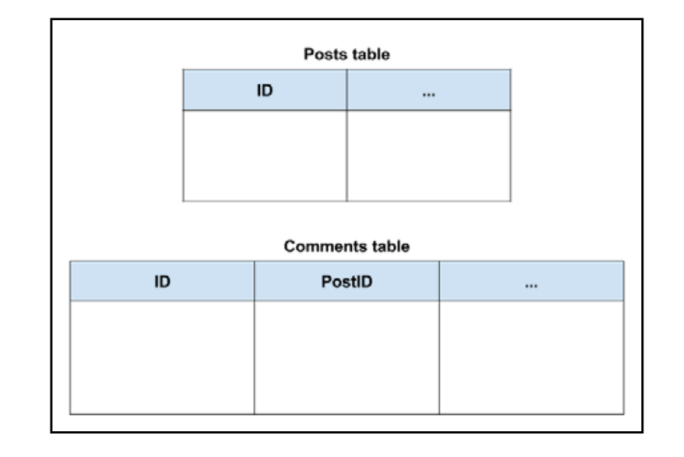
\includegraphics[scale=0.5]{sql.png}
\caption{Tabla SQL/Colección noSQL}
\end{figure}
Ejemplo de BD NoSQL:
\begin{lstlisting}
{
   "title": "First Blog Post",
   "comments": [......, ......]
}
\end{lstlisting}
Otro problema es la escalabilidad, \emph{¿qué ocurre si añadimos una nueva propiedad?}

\begin{figure}[H]
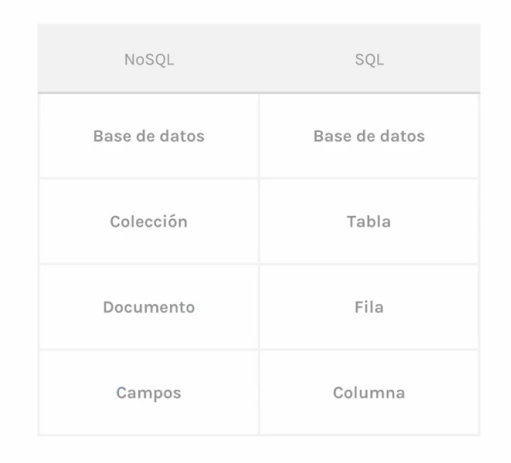
\includegraphics[scale=0.5]{noSQL.png}
\caption{Comparación SQL/noSQL}
\end{figure}

\newpage
\subsection{Características noSQL}
\begin{itemize}
\item Escalabilidad
\item Versatilidad
\item Agilidad
\item Velocidad
\end{itemize}


\subsection{BD NoSQL}
\begin{itemize}
\item MongoDB.
\item Cassandra.
\item Redis.
\item CouchDB.
\end{itemize}

\section{MongoDB}
\subsection{Introduccion}
\begin{itemize}
\item Es un sistema de base de datos NoSQL orientado a documentos, desarrollado bajo el concepto de código abierto.
\item MongoDB guarda estructuras de datos en documentos similares a JSON 
\item MongoDB utiliza una especificación llamada BSON (Binary JSON)
\item SEl desarrollo de MongoDB empezó en octubre de 2007 por la compañía de software 10gen.
\item Los drivers para los lenguajes de programación están bajo la licencia de Apache. 
\item MongoDB está escrito en C++, aunque las consultas se hacen pasando objetos JSON como parámetro.
\end{itemize}

\subsection{Características MongoDB}
\begin{itemize}
\item Alto rendimiento
\item Lenguaje de consultas avanzado
\item Alta disponibilidad
\item Escalabilidad horizontal
\item Consola de javascript
\end{itemize}

\subsection{¿Dónde se puede utilizar MongoDB?}
\begin{itemize}
\item Cualquier aplicación que necesite almacenar datos semi estructurados puede usar MongoDB.
\item Es el caso de las típicas aplicaciones CRUD o de muchos de los desarrollos web actuales.
\item MongoDB es especialmente útil en entornos que requieran escalabilidad. 
\end{itemize}

\subsection{¿Dónde no se debe usar MongoDB?}
\begin{itemize}
\item En esta base de datos no existen las transacciones. Solo garantiza operaciones atómicas a nivel de documento.Si las transacciones son algo indispensable en nuestro desarrollo, deberemos pensar en otro sistema.
\item Tampoco existen los JOINS. Para consultar datos relacionados en dos o más colecciones, tenemos que hacer más de una consulta. En general, si nuestros datos pueden ser estructurados en tablas, y necesitamos las relaciones, es mejor que optemos por un RDBMS clásico.
\item La pregunta que debemos hacernos es: ¿Cómo hacemos que el hilo ejecute código?
\end{itemize}

\section{Instalación}
Podemos instalar como servicio en el propio equipo, necesitaremos tanto servidor (\emph{mongod}) como cliente (\emph{mongo}). Pero una opción mas recomnedable es usar una imagen de \emph{docker}:
\begin{description}
\item[Servidor] \emph{docker run --name mongoServer -d mongo}
\item[Cliente] \emph{docker exec -it mongoServerAuth mongo}
\end{description}

\section{Tipo de datos}
%\begin{figure}[H]
%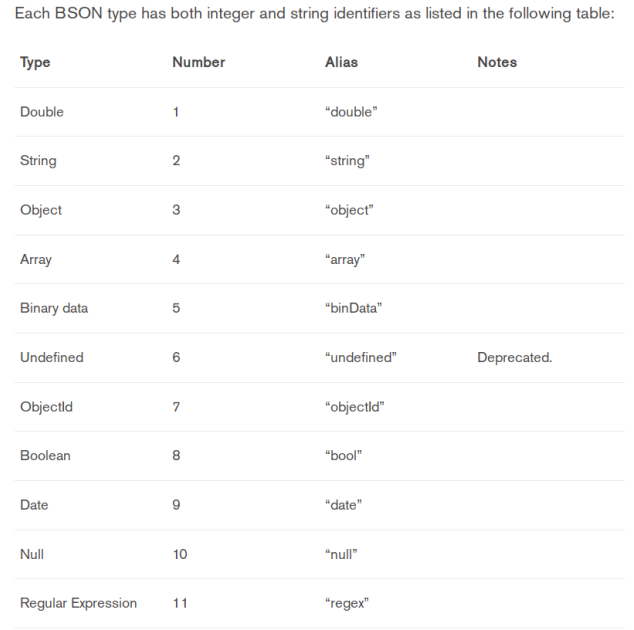
\includegraphics[scale=0.5]{tipos.png}
%\caption{Algunos tipos de datos}
%\end{figure}
\href{https://docs.mongodb.com/manual/reference/bson-types/}
{\textcolor{cyan}{\underline{Tipos datos}}}
%{\textcolor{cyan}\underline{Tipos datos}}

\newpage
\section{Operaciones CRUD}
\subsection{Introducción}
Una vez conectado al servidor podremos realizar operaciones tales como:
\begin{description}
\item[Mostrar las BD] \emph{show dbs}
\item[Crear una BD] \emph{use nombreBD}, también utilizamos este comando para conectarnos a una BD existente.
\item[Mostrar las colecciones de la BD] \emph{show collections}
\item[Borrar la BD] \emph{db.dropDatabase()}  estándo en uso de la BD
\end{description}

\subsection{Creando colecciones}
Podemos usar estos comandos:
\begin{itemize}
\item \emph{db.createCollection()} definimos el nombre de la colección y sus propiedades.
\item \emph{db.nombreColeccion.insert()} damos el nombre (\emph{nombreColeccion}) e insertamos un documento.
\end{itemize}

\subsubsection{Características de los documentos}
\begin{itemize}
\item No tienen estructura definida
\item Formato \emph{JSON}
\item Se almacena en documentos
\item Par \emph{clave/valor}
\item La clave primaria es \emph{\-id}
\end{itemize}
\begin{figure}[H]
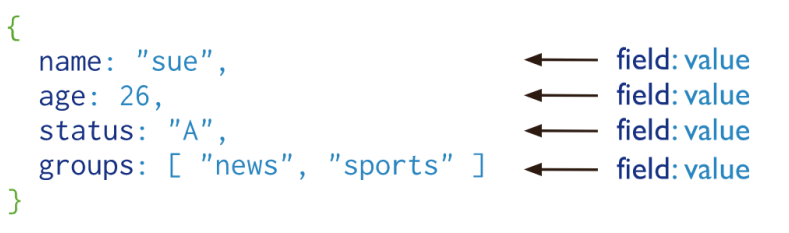
\includegraphics[scale=0.5]{documentos.png}
\caption{Ejemplo de documento}
\end{figure}

\subsubsection{createCollection}
Tenemos como opciones:
\begin{description}
\item[capped] puede ser \emph{true o false}, que define la colección de tipo \emph{capped collection} y podemos indicar su tamaño.
\item[autoIndex] \emph{true o false} para especificar el uso \emph{\_id}
\item[max] número que indica el máximo de documentos de una colección.
\item[validator] define las validaciones de cada campo.
\end{description}

\begin{lstlisting}
db.createCollection( "contacts",
   { validator: { $or:
      [
         { phone: { $type: "string" } },
         { email: { $regex: /@mongodb\.com$/ } },
         { status: { $in: [ "Unknown", "Incomplete" ] } }
      ]
   }
} )
\end{lstlisting}

\subsubsection{Insertando documentos}
\begin{lstlisting}
> use bd
switched to db bd
> db.coleccion.insert({_id : 1, nombre: 'federico' , edad : 34});
WriteResult({ "nInserted" : 1 })
> 
\end{lstlisting}

\newpage

\subsubsection{Lectura de documentos}
MongoDB permite:
\begin{itemize}
\item Proyectar algunos documentos.
\item Aplicar expresiones regulares en la búsqueda
\item Ordenar la búsqueda
\item Limitar el número de resultado.
\item Usar \emph{pretty()}
\end{itemize}

Los datos con lo que vamos a trabajar son:

\begin{lstlisting}
[{"ciudad":"Angatel","pais":"Philippines","zonaHoraria":"Asia/Manila","latitud":15.8137804,"longitud":120.3404633},
{"ciudad":"Panggungrejo","pais":"Indonesia","zonaHoraria":"Asia/Jakarta","latitud":-7.6385033,"longitud":112.9148168},
{"ciudad":"Osilnica","pais":"Slovenia","zonaHoraria":"Europe/Zagreb","latitud":45.5291637,"longitud":14.6984205},
{"ciudad":"Barrosa","pais":"Portugal","zonaHoraria":"Europe/Lisbon","latitud":38.9587954,"longitud":-8.755077},
{"ciudad":"Bongbong","pais":"Indonesia","zonaHoraria":"Asia/Jakarta","latitud":"-6.3943","longitud":"105.9495"},
{"ciudad":"Bacabal","pais":"Brazil","zonaHoraria":"America/Fortaleza","latitud":-4.2221443,"longitud":-44.7855844},
{"ciudad":"Ujazd","pais":"Poland","zonaHoraria":"Europe/Warsaw","latitud":51.6113555,"longitud":19.8982345},
{"ciudad":"Cabungan","pais":"Philippines","zonaHoraria":"Asia/Manila","latitud":16.289185,"longitud":119.90559},
{"ciudad":"San Ignacio","pais":"Honduras","zonaHoraria":"America/Tegucigalpa","latitud":14.6546241,"longitud":-87.0399404},
{"ciudad":"Webuye","pais":"Kenya","zonaHoraria":"Africa/Nairobi","latitud":0.5992059,"longitud":34.779603}, ...
\end{lstlisting}

Importando un fichero con un \emph{array} de \emph{json}, obtenido de la página de \emph{mockaroo}
\begin{lstlisting}
//CREAMOS CONTENEDOR MONGO
docker run --name mongo-server -d mongo
//COPIAMOS FICHERO ARRAY JSON AL CONTENEDOR
docker cp datos.json mongo-server:/tmp/movies.json
//EJECUTAMOS MONGOIMPORT PARA COPIAR LOS DATOS DEL ARRAY JSON A LA BASE DE DATOS
docker exec -it mongo-server  mongoimport --db ejemplo --collection geografia --file /tmp/geografia.json --jsonArray
//ARRANCAMOS UN CLIENTE PARA CONECTARNOS AL SERVIDOR
docker exet -it mongoServer mongo
\end{lstlisting}

\newpage

Podemos mostrar todos los documentos:
\begin{lstlisting}
> use ejemplo
switched to db ejemplo
> show collections
geografia
> db.geografia.find().pretty().limit(3)
{
	"_id" : ObjectId("5db861810aad49beee9f1fde"),
	"ciudad" : "Barrosa",
	"pais" : "Portugal",
	"zonaHoraria" : "Europe/Lisbon",
	"latitud" : 38.9587954,
	"longitud" : -8.755077
}
{
	"_id" : ObjectId("5db861810aad49beee9f1fdf"),
	"ciudad" : "Bongbong",
	"pais" : "Indonesia",
	"zonaHoraria" : "Asia/Jakarta",
	"latitud" : "-6.3943",
	"longitud" : "105.9495"
}
{
	"_id" : ObjectId("5db861810aad49beee9f1fe0"),
	"ciudad" : "Panggungrejo",
	"pais" : "Indonesia",
	"zonaHoraria" : "Asia/Jakarta",
	"latitud" : -7.6385033,
	"longitud" : 112.9148168
}
\end{lstlisting}

Proyectando algunos campos: (El \_id no se muestra)
Podemos mostrar todos los documentos:
\begin{lstlisting}
> db.geografia.find({}, {latitud : 1, longitud : 1, _id : 0}).limit(3)
{ "latitud" : 38.9587954, "longitud" : -8.755077 }
{ "latitud" : "-6.3943", "longitud" : "105.9495" }
{ "latitud" : -7.6385033, "longitud" : 112.9148168 }
\end{lstlisting}

Mostrar títulos usando una expresión regular, mostramos las películas que empiezan por P ó S
\begin{lstlisting}
> db.movies.find({title: {$regex: '^[PS]'}});
{ "_id" : 5, "title" : "Philadelphia Experiment, The", "genre" : [ "Adventure,Drama,Sci-Fi" ] }
{ "_id" : 6, "title" : "Paranormal Activity 3", "genre" : [ "Horror" ] }
{ "_id" : 7, "title" : "Star 80", "genre" : [ "Drama" ] }
{ "_id" : 12, "title" : "Saved!", "genre" : [ "Comedy,Drama" ] }
{ "_id" : 19, "title" : "Solstice", "genre" : [ "Drama" ] }
{ "_id" : 10, "title" : "Seaside (Bord de Mer)", "genre" : [ "Drama" ] }
> 
\end{lstlisting}

\newpage
Consultando todos los documentos y listando los ocho primeros:
\begin{lstlisting}
> db.geografia.find( {ciudad : {$regex : '^[AZ]'}}, {ciudad : 1, pais : 1, _id : 0}).limit(8)
{ "ciudad" : "Angatel", "pais" : "Philippines" }
{ "ciudad" : "Alexandria", "pais" : "United States" }
{ "ciudad" : "Antsirabe", "pais" : "Madagascar" }
{ "ciudad" : "Alikalia", "pais" : "Sierra Leone" }
{ "ciudad" : "Agustin Codazzi", "pais" : "Colombia" }
{ "ciudad" : "Alcaria", "pais" : "Portugal" }
{ "ciudad" : "Ayagoz", "pais" : "Kazakhstan" }
{ "ciudad" : "Zherdevka", "pais" : "Russia" }
\end{lstlisting}

Además ordenada alfabéticamente:
\begin{lstlisting}
> db.geografia.find({},  {ciudad : 1, pais : 1, _id : 0}).sort({pais : 1}).limit(5)
{ "ciudad" : "Ghormach", "pais" : "Afghanistan" }
{ "ciudad" : "Qarah Bagh", "pais" : "Afghanistan" }
{ "ciudad" : "Ghurayd Gharame", "pais" : "Afghanistan" }
{ "ciudad" : "Kabul", "pais" : "Afghanistan" }
{ "ciudad" : "Muta Khan", "pais" : "Afghanistan" }
\end{lstlisting}

Además ordenada alfabéticamente a la inversa:
\begin{lstlisting}
> db.geografia.find({},  {ciudad : 1, pais : 1, _id : 0}).sort({pais : -1}).limit(5)
{ "ciudad" : "Redcliff", "pais" : "Zimbabwe" }
{ "ciudad" : "Chipata", "pais" : "Zambia" }
{ "ciudad" : "Maswarah", "pais" : "Yemen" }
{ "ciudad" : "Yufrus", "pais" : "Yemen" }
{ "ciudad" : "Suq ar Rabu", "pais" : "Yemen" }
\end{lstlisting}

Buscando en un campo de tipo \emph{cadena}
\begin{lstlisting}
> db.geografia.find({pais : 'Spain'} , {_id: 0})
{ "ciudad" : "Toledo", "pais" : "Spain", "zonaHoraria" : "Europe/Madrid", "latitud" : 39.873363, "longitud" : -4.0414005 }
{ "ciudad" : "Palma De Mallorca", "pais" : "Spain", "zonaHoraria" : "Europe/Madrid", "latitud" : 39.609109, "longitud" : 2.6362975 }
{ "ciudad" : "Vigo", "pais" : "Spain", "zonaHoraria" : "Europe/Madrid", "latitud" : 42.229169, "longitud" : -8.7026991 }
\end{lstlisting}


\newpage
\subsubsection{Borrando documentos}
Podemos usar:
\begin{itemize}
\item remove, elimina uno o varios documentos
\item drop, borra una coleccion \emph{db.coleccion.drop()}
\end{itemize}
Borrando de documentos registro:
\begin{lstlisting}
db.collection.remove(
   <query>,
   <justOne>
)
\end{lstlisting}
Donde:
\begin{description}
\item[query] Especifica el criterio de borrado, sino se especifica puede borrar todos los documentos. Cambia a partir de la versión 2.6 y no borra todos.
\item[justOne] Es opcional, puede ser \emph{true o false}, por defecto es \emph{false} y borra todos los documentos que encaje con la búsqueda
\end{description}
Borrando todos los registros:
\begin{lstlisting}
> db.geografia.drop();
true
> 
\end{lstlisting}

\begin{lstlisting}
> db.geografia.find({pais : {$regex : '^S'}}).count()
71
db.geografia.remove({pais : {$regex : '^S'}})
WriteResult({ "nRemoved" : 71 })
> db.geografia.find({pais : {$regex : '^S'}}).count()
0
> db.geografia.find({pais : {$regex : '^A'}}).count()
35
> db.geografia.remove({pais : {$regex : '^A'}}, true)
WriteResult({ "nRemoved" : 1 })
> db.geografia.find({pais : {$regex : '^A'}}).count()
34
\end{lstlisting}

\subsubsection{Actualizando documentos}
\begin{lstlisting}
db.collection.update(
   <query>,
   <update>,
   {
     upsert: <boolean>,
     multi: <boolean>,
     writeConcern: <document>,
     collation: <document>,
     arrayFilters: [ <filterdocument1>, ... ],
     hint:  <document|string>        // Available starting in MongoDB 4.2
   }
)
\end{lstlisting}
\begin{description}
\item[query] El criterio de selección.
\item[update] La modificación a ejecutar.
\item[upsert] Puede ser \emph{true o false}. En el caso de \emph{true} crea un nuevo documento si el criterio de selección no encaja con ningún documento. El valor por defecto es \emph{false}
\item[multi] Puede ser \emph{true o false}. En el caso de \emph{true} modifica todos los documentos si el criterio de selección no encaja con ningún documento. El valor por defecto es \emph{false}
\end{description}
Tenemos operadores como:


\begin{lstlisting}
> db.geografia.find({pais : 'Germany'}, {_id : 0}).count()
4
> db.geografia.update({pais : 'Germany' }, {pais: 'Alemania'})
WriteResult({ "nMatched" : 1, "nUpserted" : 0, "nModified" : 1 })
> db.geografia.find({pais : 'Germany'}, {_id : 0}).count()
3
> db.geografia.find({pais : 'Alemania'}, {_id : 0}).count()
1
> db.geografia.find({pais : 'Alemania'})
{ "_id" : ObjectId("5db861810aad49beee9f208d"), "pais" : "Alemania" }
> db.geografia.find({pais : 'Germany'}, {_id : 0})
{ "ciudad" : "Dortmund", "pais" : "Germany", "zonaHoraria" : "Europe/Berlin", "latitud" : 51.4918437, "longitud" : 7.5319762 }
{ "ciudad" : "Bonn", "pais" : "Germany", "zonaHoraria" : "Europe/Berlin", "latitud" : 50.7074591, "longitud" : 7.1093481 }
{ "ciudad" : "Wurzburg", "pais" : "Germany", "zonaHoraria" : "Europe/Berlin", "latitud" : 49.8180135, "longitud" : 9.9637931 }
\end{lstlisting}

\newpage

\begin{description}
\item[\$inc] incrementa un valor numérico.
\item[\$rename] renombra el nombre de una clave
\item[\$set] para actualizar solo un campo
\end{description}

\begin{lstlisting}
> db.geografia.find({pais : 'Greece'}, {_id : 0})
{ "ciudad" : "Portaria", "pais" : "Greece", "zonaHoraria" : "Europe/Athens", "latitud" : 39.3897164, "longitud" : 22.9982253 }
{ "ciudad" : "Oropos", "pais" : "Greece", "zonaHoraria" : "Europe/Athens", "latitud" : 38.3032384, "longitud" : 23.7548814 }
{ "ciudad" : "Filiates", "pais" : "Greece", "zonaHoraria" : "Europe/Athens", "latitud" : 39.6003316, "longitud" : 20.3077691 }
{ "ciudad" : "Elaiochori", "pais" : "Greece", "zonaHoraria" : "Europe/Athens", "latitud" : 40.8207633, "longitud" : 24.2429692 }
{ "ciudad" : "Zevgolateio", "pais" : "Greece", "zonaHoraria" : "Europe/Athens", "latitud" : 37.9375856, "longitud" : 22.8008984 }
{ "ciudad" : "Karatoulas", "pais" : "Greece", "zonaHoraria" : "Europe/Athens", "latitud" : 37.4703686, "longitud" : 22.1773357 }
{ "ciudad" : "Kassandreia", "pais" : "Greece", "zonaHoraria" : "Europe/Athens", "latitud" : 40.0480392, "longitud" : 23.4134501 }
> db.geografia.update( {pais : 'Greece'}, {$set: { pais : 'Grecia' }}, {multi: true} )
WriteResult({ "nMatched" : 7, "nUpserted" : 0, "nModified" : 7 })
> db.geografia.find({pais : 'Grecia'}, {_id : 0})
{ "ciudad" : "Portaria", "pais" : "Grecia", "zonaHoraria" : "Europe/Athens", "latitud" : 39.3897164, "longitud" : 22.9982253 }
{ "ciudad" : "Oropos", "pais" : "Grecia", "zonaHoraria" : "Europe/Athens", "latitud" : 38.3032384, "longitud" : 23.7548814 }
{ "ciudad" : "Filiates", "pais" : "Grecia", "zonaHoraria" : "Europe/Athens", "latitud" : 39.6003316, "longitud" : 20.3077691 }
{ "ciudad" : "Elaiochori", "pais" : "Grecia", "zonaHoraria" : "Europe/Athens", "latitud" : 40.8207633, "longitud" : 24.2429692 }
{ "ciudad" : "Zevgolateio", "pais" : "Grecia", "zonaHoraria" : "Europe/Athens", "latitud" : 37.9375856, "longitud" : 22.8008984 }
{ "ciudad" : "Karatoulas", "pais" : "Grecia", "zonaHoraria" : "Europe/Athens", "latitud" : 37.4703686, "longitud" : 22.1773357 }
{ "ciudad" : "Kassandreia", "pais" : "Grecia", "zonaHoraria" : "Europe/Athens", "latitud" : 40.0480392, "longitud" : 23.4134501 }
\end{lstlisting}

\newpage

\subsection{Ejercicio}
\begin{itemize}
\item Borra la colección con la que has trabajado en este documento.
\item Vuelve a cargar dicha colección.
\item Muestra el número de documentos de la colección.
\item Realiza una búsqueda de los documentos que se encuentre en el hemisferio sur (latitud negativa). Realiza una proyección para que solo se muestre el nombre de la ciudad y del país.
\item Añade a la consulta anterior, que además se encuentra en el oeste del meridiano de \emph{Greenwich}, es decir longitud negativa.
\item Realiza una consulta similiar, pero que  nos diga los documentos que son ciudades de paises que son o bien del hemisferio norte o sean ciudades de paises del este.
\item Inserta el dato de Jáen, usa como pais España.
\item Actualiza este último registro para cambiar el nombre de España por Spain.
\item Actualiza todos los paises que empiezan por vocal, para que cambie el nombre de ciudad, por \emph{ciudad que empieza por vocal}
\item Borra todos estos últimos documentos modificados, incluye el de Jaén también.
\end{itemize}

\end{document}
